% Original teaching figure: same physical coordinate scales in both panels.
\documentclass[tikz,border=3mm]{standalone}
\begin{document}
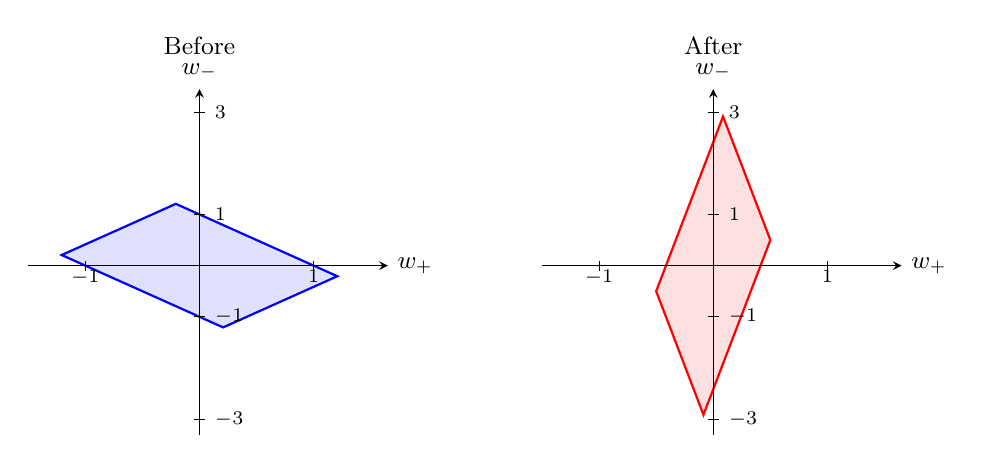
\begin{tikzpicture}[>=stealth,font=\small,x=1.45cm,y=.65cm]
\foreach \offset/\title in {0/Before,4.5/After} {
\begin{scope}[shift={(\offset,0)}]
\ifdim\offset pt=0pt
\draw[blue,thick,fill=blue!12] (1.207107,-.207107)--(-.207107,1.207107)--(-1.207107,.207107)--(.207107,-1.207107)--cycle;
\else
\draw[red,thick,fill=red!12] (.5,.5)--(-.085786,-2.914214)--(-.5,-.5)--(.085786,2.914214)--cycle;
\fi
\draw[->] (-1.5,0)--(1.65,0) node[right] {$w_+$};
\draw[->] (0,-3.3)--(0,3.45) node[above] {$w_-$};
\foreach \y in {-3,-1,1,3} {\draw (-.05,\y)--(.05,\y) node[right] {\scriptsize$\y$};}
\foreach \x in {-1,1} {\draw (\x,-.1)--(\x,.1) node[below] {\scriptsize$\x$};}
\node at (0,4.3) {\title};
\end{scope}
}
\end{tikzpicture}
\end{document}
